
\section{Anforderungsspezifikation}
\label{Anforderungsspezifikation}

\subsection{Use Cases}
\label{Anforderungsspezifikation:Use Cases}

Im folgenden sind die funktionalen Anforderungen an das System mit all seinen Komponenten, welche im Kapitel \ref{Architektur} aufgeführt sind, als Use Cases im Brief-Format beschrieben. 
Zur Übersicht ist das Use Case Diagramm in Abbildung \ref{fig:UseCase_OeV-Gueteklassen_2018} zu betrachten.

\begin{figure}[ht]
\centering
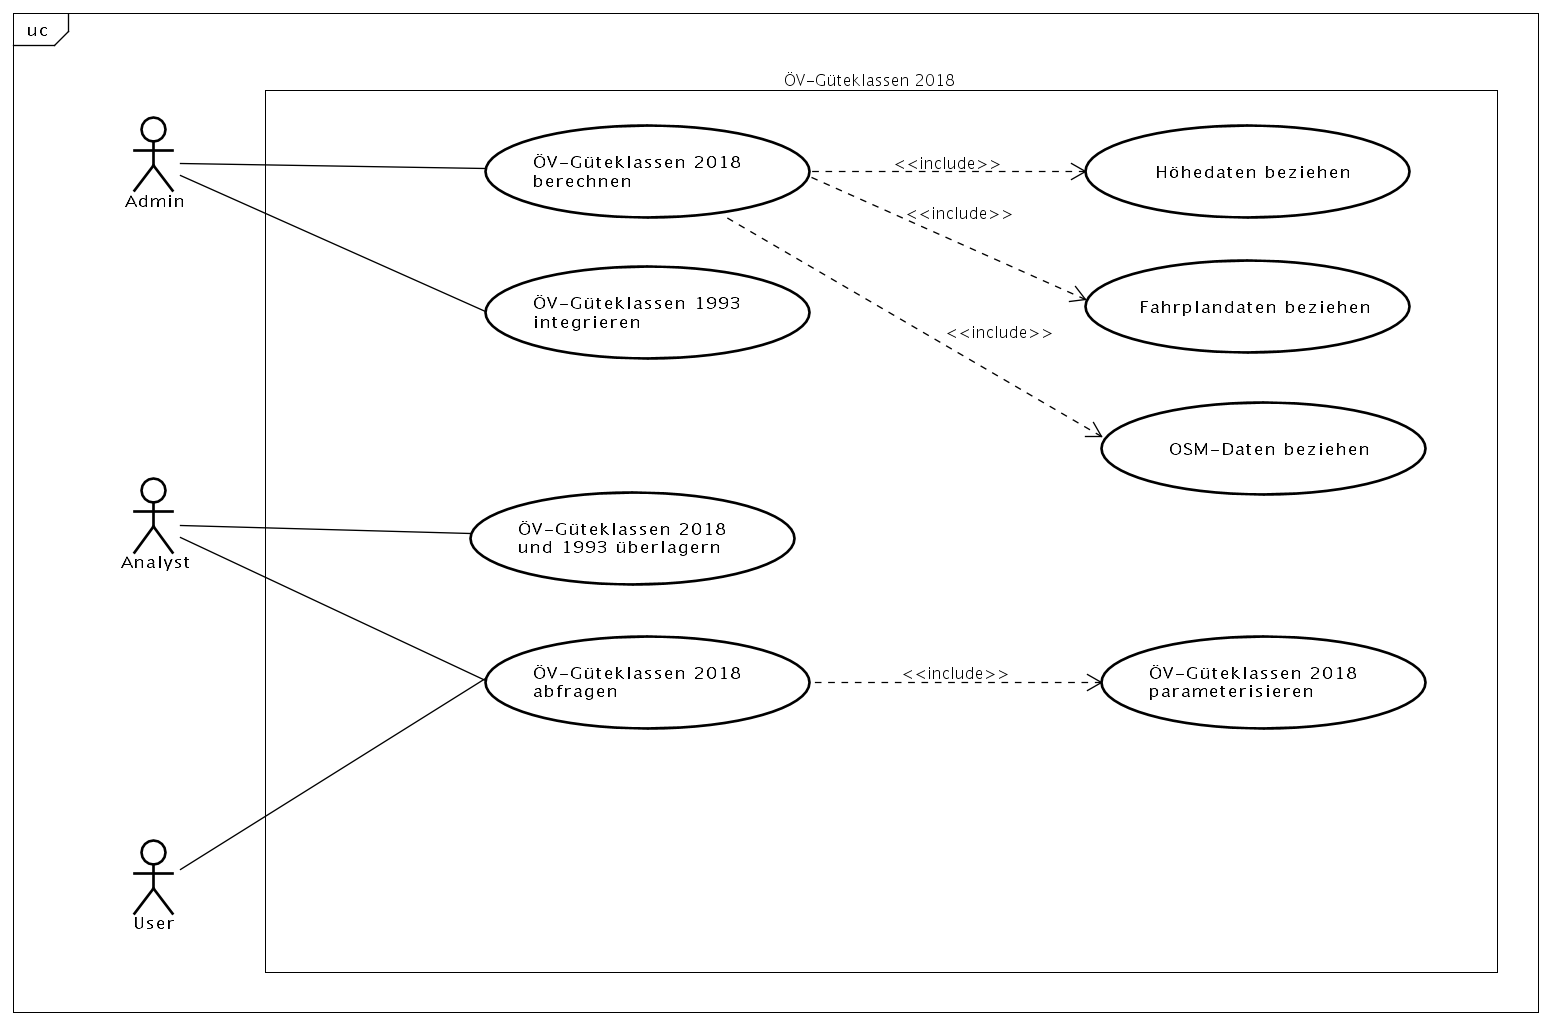
\includegraphics[width=0.7\linewidth]{projectdoc/img/UseCase_OeV-Gueteklassen_2018}
\caption[Use Case Diagramm]{Use Case Diagramm}
\label{fig:UseCase_OeV-Gueteklassen_2018}
\end{figure}

\subsubsection{Aktoren}
\label{Use Cases:Aktoren}

Um die Anforderungen akkurat evaluieren zu können, ist es essentiell dass die Aktoren des Systems identifiziert werden. 
In der Tabelle der Tabelle \ref{table:aktoren} sind die Aktoren mit ihren Interessen aufgelistet. 

\begin{table}[h]
    \centering
    \caption{Aktoren}
    \label{table:aktoren}
    \begin{tabular}{ll}
        \textbf{Aktor} & \textbf{Beschreibung und Interessen}                                                                                                                                                                                     \\
        \textbf{User}  & \begin{tabular}[c]{@{}l@{}}Ein User ist ...\end{tabular}                                          \\
        \textbf{Admin} & \begin{tabular}[c]{@{}l@{}}Ein Admin ist ...\end{tabular}
    \end{tabular}
\end{table}

\subsubsection{UC01: TODO}
\label{Use Cases:UC01}

Aktoren: \emph{User}

Include: \nameref{Use Cases:UC02}

%TODO

\subsubsection{UC02: TODO}
\label{Use Cases:UC02}

Aktoren: \emph{User}

%TODO


\subsection{Nicht-funktionale Anforderungen}
\label{Anforderungsspezifikation:Nicht-funktionale Anforderungen}

\subsubsection{NFA01: TODO}
\label{NFA:NFA01}

%TODO

